
%%%%%%%%%%%%%%%%%%%%%%%%%%%%%%%%%%%%%%%%%%%%%%%%%%%%%%%%%%%%%%%%%%%%%%%%%%%%%%%%
%% SECTION
%%%%%%%%%%%%%%%%%%%%%%%%%%%%%%%%%%%%%%%%%%%%%%%%%%%%%%%%%%%%%%%%%%%%%%%%%%%%%%%%
\section{\textcolor{blue}{Historia da samba de gafieira}}
\index{Historia da samba de gafieira}


O samba de gafieira, como dança, descende principalmente do maxixe (dança),
que a sua vez foi gerado  pela união do  lundu, 
a polca e outras danças europeias.
Assim, misturando o maxixe com a ginga, e o ritmo de outras danças africanas, 
é que se obteve o que agora chamaríamos como samba de gafieira primigênio \cite[pp. 139]{perna2002samba}.


O aparecimento do samba nos salões de dança, 
foi um grande impacto para as pessoas que frequentavam estes lugares;
sendo considerado um ritmo novo e ligeiro,
que desagradou aos bailarinos de maior idade e menos ágeis \cite[pp. 3]{entrevistajuliojournalbrasil1}.
O senhor, Júlio Simões, socio da ``Kananga do Japão'' e
do ``Elite Club'', chegou a temer pelo futuro do seus empreendimentos; porem, para sorte dele, 
o samba fez muito sucesso no Elite,
e passou a ser considerado matéria indispensável para qualquer pessoa que pretendesse ser bailarino, 
compositor ou instrumentista \cite[pp. 3]{entrevistajuliojournalbrasil1}.

Pode-se estabelecer o ingresso do samba, aos salões de dança, entre os anos de 1930 e 1940 \cite[pp. 140]{perna2002samba}.
Para o ano de 1940 o samba dançado em salões, já tinha ganhado muita força;
porem, podia-se ver 3 formas diferentes de ser dançado \cite[pp. 142-143]{perna2002samba}:
\begin{itemize}
\item \textbf{Samba-canção}, que agora é um modo extinto \cite[pp. 143]{perna2002samba},
\item \textbf{Samba-batucada}, que é esse samba de gafieira primigênio \cite[pp. 143]{perna2002samba}, e
\item \textbf{Samba liso}, que é um estilo de dança que perdura ainda ate nosso dias \cite[pp. 143]{perna2002samba}, ver Seção \ref{subsec:estilosdedanca}.
\end{itemize}
Com o passar dos anos foram agregados elementos de outras danças a esse samba de gafieira primigênio;
por exemplo, movimentos do tango e do rock.

A Figura \ref{fig:formuladosambagafieira} mostra o árvore genealógico de nosso samba de gafieira atual.
\begin{figure}[h]
  \centering
    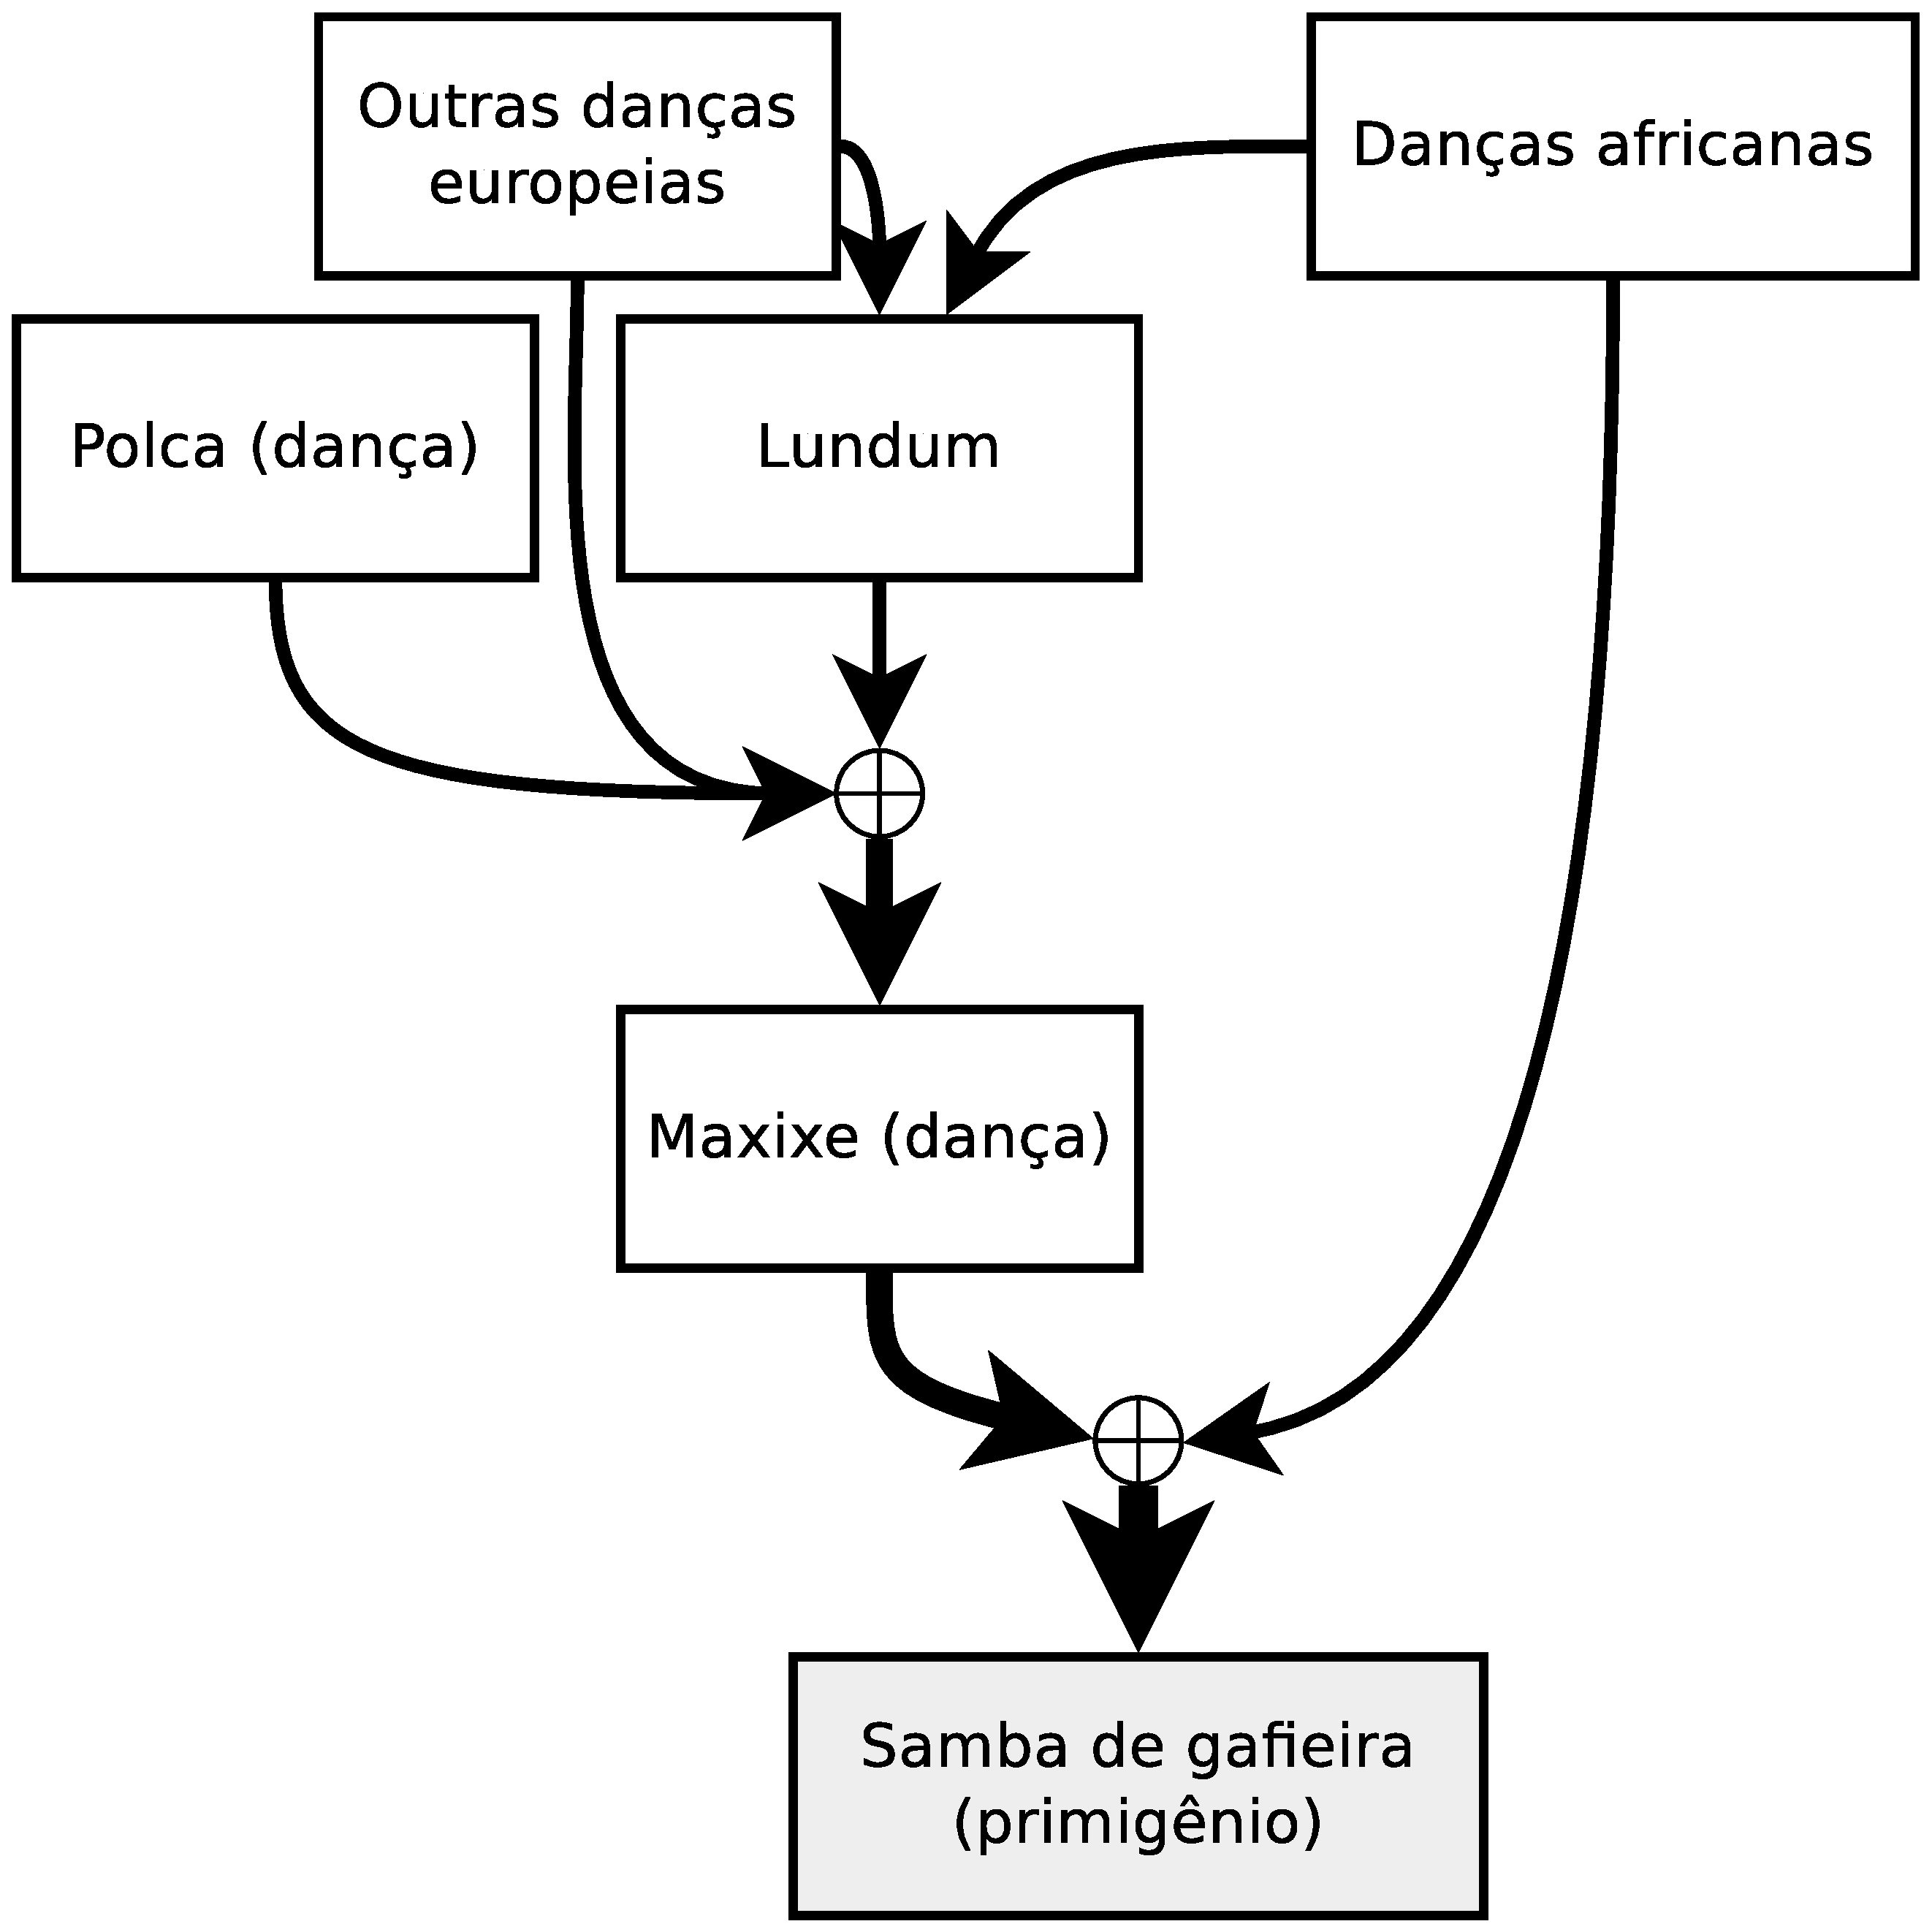
\includegraphics[width=0.6\textwidth]{chapters/cap-historia/sambagafieiraformula.eps}
  \caption{Formula da criação do samba de gafieira.}
\label{fig:formuladosambagafieira}
\end{figure}

\subsection{Em que estilos musicais posso dançar samba de gafieira?}
\label{subsec:gafieiradancaestilos}

Entre os estilos musicais em que o samba de gafieira se adapta bem, temos:
\begin{itemize}
\item \textbf{Samba de gafieira}
\item \textbf{Samba de breque}
\item \textbf{Pagode paulista}
\item \textbf{Partido alto}
\item \textbf{Pagode carioca}
\item \textbf{Samba canção}
\item \textbf{Bossa nova}
\item \textbf{Choro}.
%\item \textbf{}
\end{itemize}

A Figura \ref{fig:gafieiradancaestilos} mostra um resumo dos 
tipos de estilos musicais onde pode ser dançado samba de gafieira.
\begin{figure}[h]
  \centering
    \includegraphics[width=0.6\textwidth]{chapters/cap-historia/gafieiravcmusica.eps}
  \caption{ Estilos de músicas no samba onde pode-se dançar samba de gafieira.}
\label{fig:gafieiradancaestilos}
\end{figure}


